\frame{\frametitle{Double-diffusive convection defines instabilities in nominally stable fluids with two opposing buoyant fields.}
\begin{overprint}
	\only<1>{
	\begin{figure}[h]
		\centering
			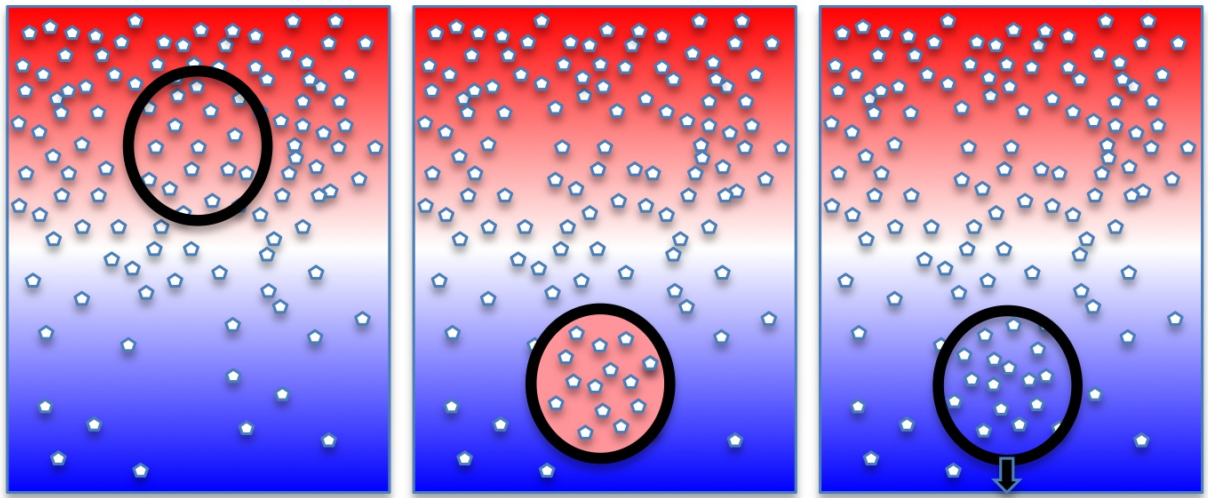
\includegraphics[width=.9\textwidth]{fingdiagram.png}\footnote{\citep{Garaud2014}}
		\label{fig:figs_scdiagram}
		\caption{Fingering (FC; also Thermohaline, Thermocompositional) Convection}
	\end{figure}}
	\only<2>{
	\begin{figure}[h]
		\centering
			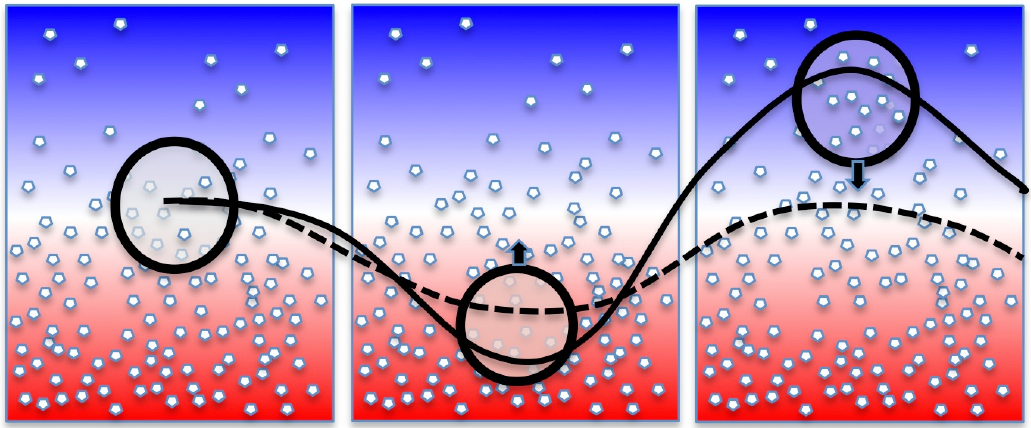
\includegraphics[width=.9\textwidth]{scdiagram.png}\footnote{\citep{Garaud2014}}
		\label{fig:figs_scdiagram}
		\caption{Oscillatory Double-Diffusive Convection (ODDC; also sometimes Semi-Convection)}
	\end{figure}}
\end{overprint}
}

% \frame{\frametitle{ODDC is modeled in stars using the \citet{Langer1983} prescription by deriving a diffusion coefficient, $D$.}
% \begin{columns}
% 	\column{150pt}
% 	{\bf MESA \citep{Langer1983}}
% 	\begin{itemize}
% 		\item Only mixes composition
% 		\item One free parameter, $\alpha$
% 	\end{itemize}
% 	\begin{align}
% 		D=&\frac{\alpha \kappa_{T}}{6}\frac{\frac{dT}{dz}-\left.\frac{\partial T}{\partial z}\right|_{\rm{ad}}}{\frac{\phi T}{\delta \mu}\frac{d\mu}{dz}+\left.\frac{\partial T}{\partial z}\right|_{\rm{ad}}-\frac{dT}{dz}} \\
% 		\delta\equiv&-\frac{\partial \ln\rho}{\partial\ln T}, \phi\equiv\frac{\partial\ln\rho}{\partial\ln\mu}
% 	\end{align}
% 	\column{150pt}
% 	{\bf KEPLER \citep{Woosley1988}}
% 	\begin{itemize}
% 		\item Only mixes composition
% 		\item One free parameter, $F$
% 	\end{itemize}
% 	\begin{equation}
% 		D=\frac{F\kappa_{T}D_{b}}{F\kappa_{T}+D_{b}}
% 	\end{equation}
% 	\begin{equation}
% 		D_{b}\propto\left(\frac{dT}{dz}-\left.\frac{\partial T}{\partial z}\right|_{\rm{ad}}\right)^{\frac{1}{2}}
% 	\end{equation}
% \end{columns}
% }

% \frame{\frametitle{In particular, ODDC has strong relevance to stellar evolution because stellar cores are hot and heavy \citep{Robertson1972}.}
% 	\begin{figure}[h]
% 			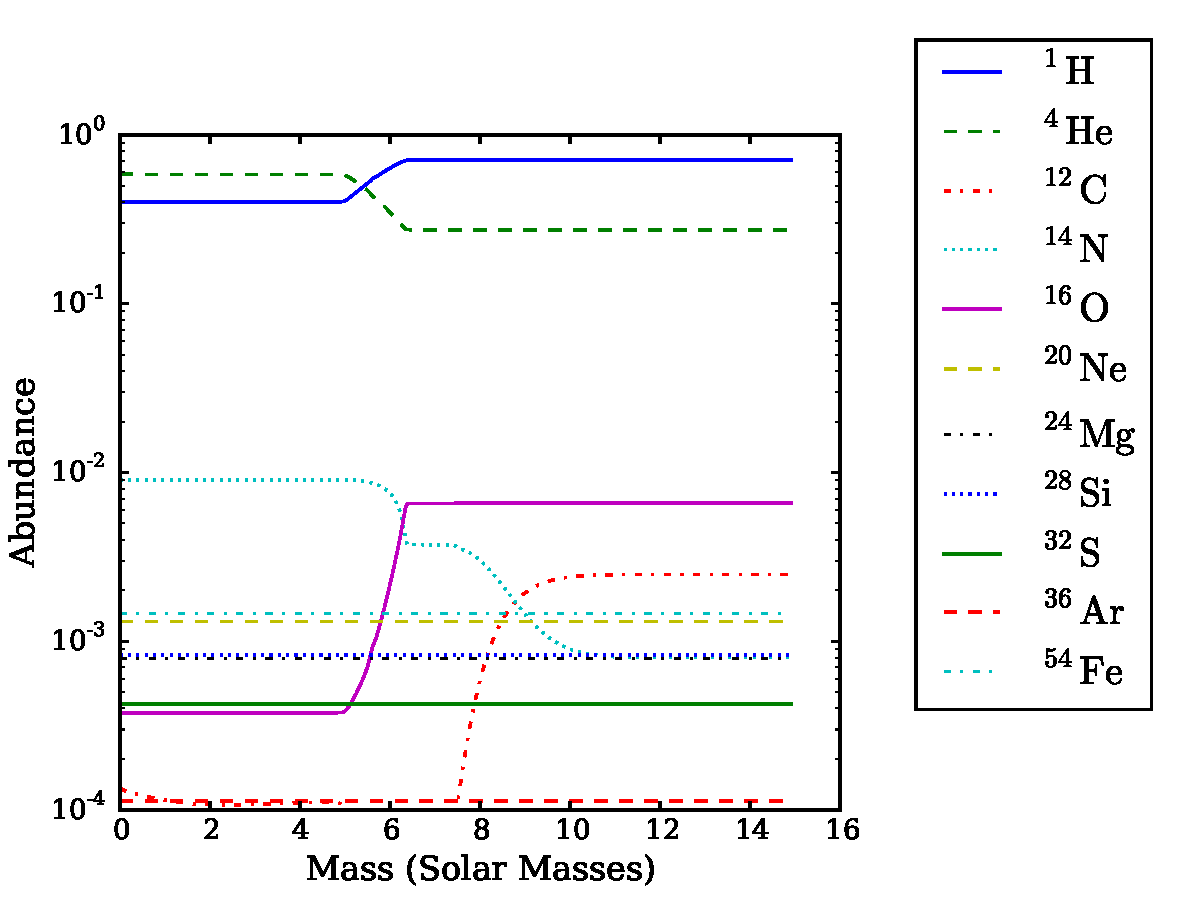
\includegraphics[width=.5\textwidth]{hburn_abun.pdf}
% 			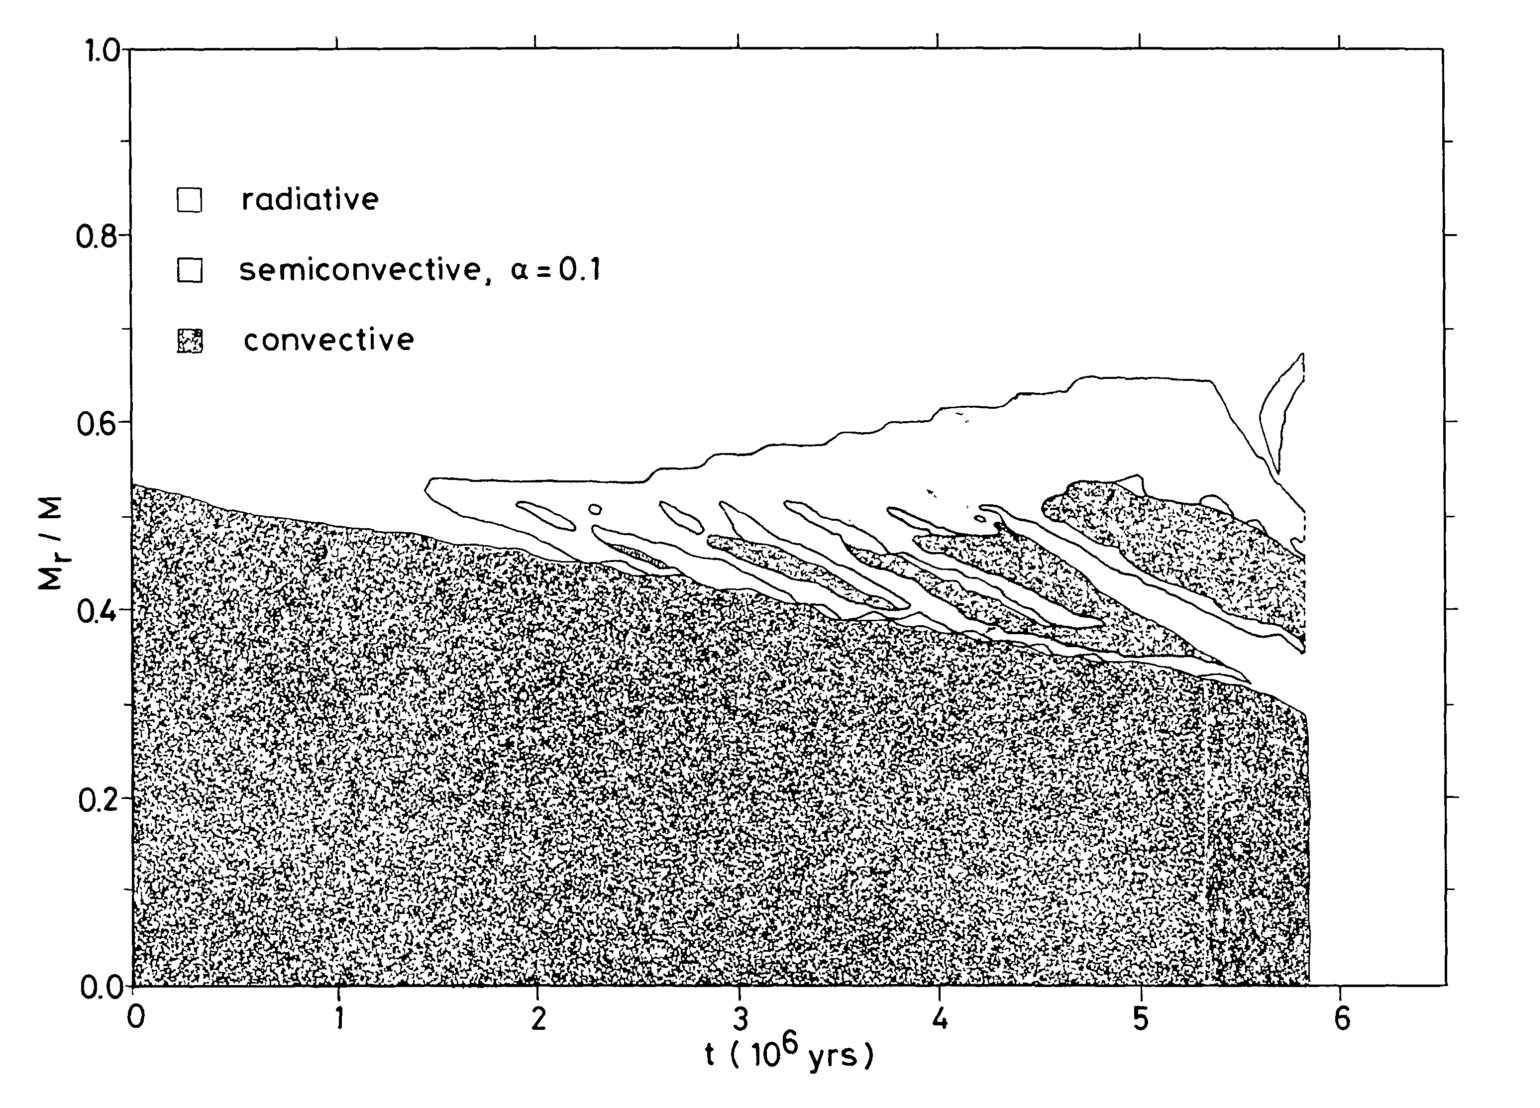
\includegraphics[width=.5\textwidth]{figs/Langer-core-sc.png}\footnote{\citep{Langer1985}}
% 		\label{fig:figs_Langer-core-sc}
% 	\end{figure}
% }

% \frame{\frametitle{We have in the past extracted flux laws for one form: homogenous fingering convection.}
% \begin{figure}
% 	\caption{Plotting, $\tilde{\mu}$, the perturbation of the mean molecular weight.}
% 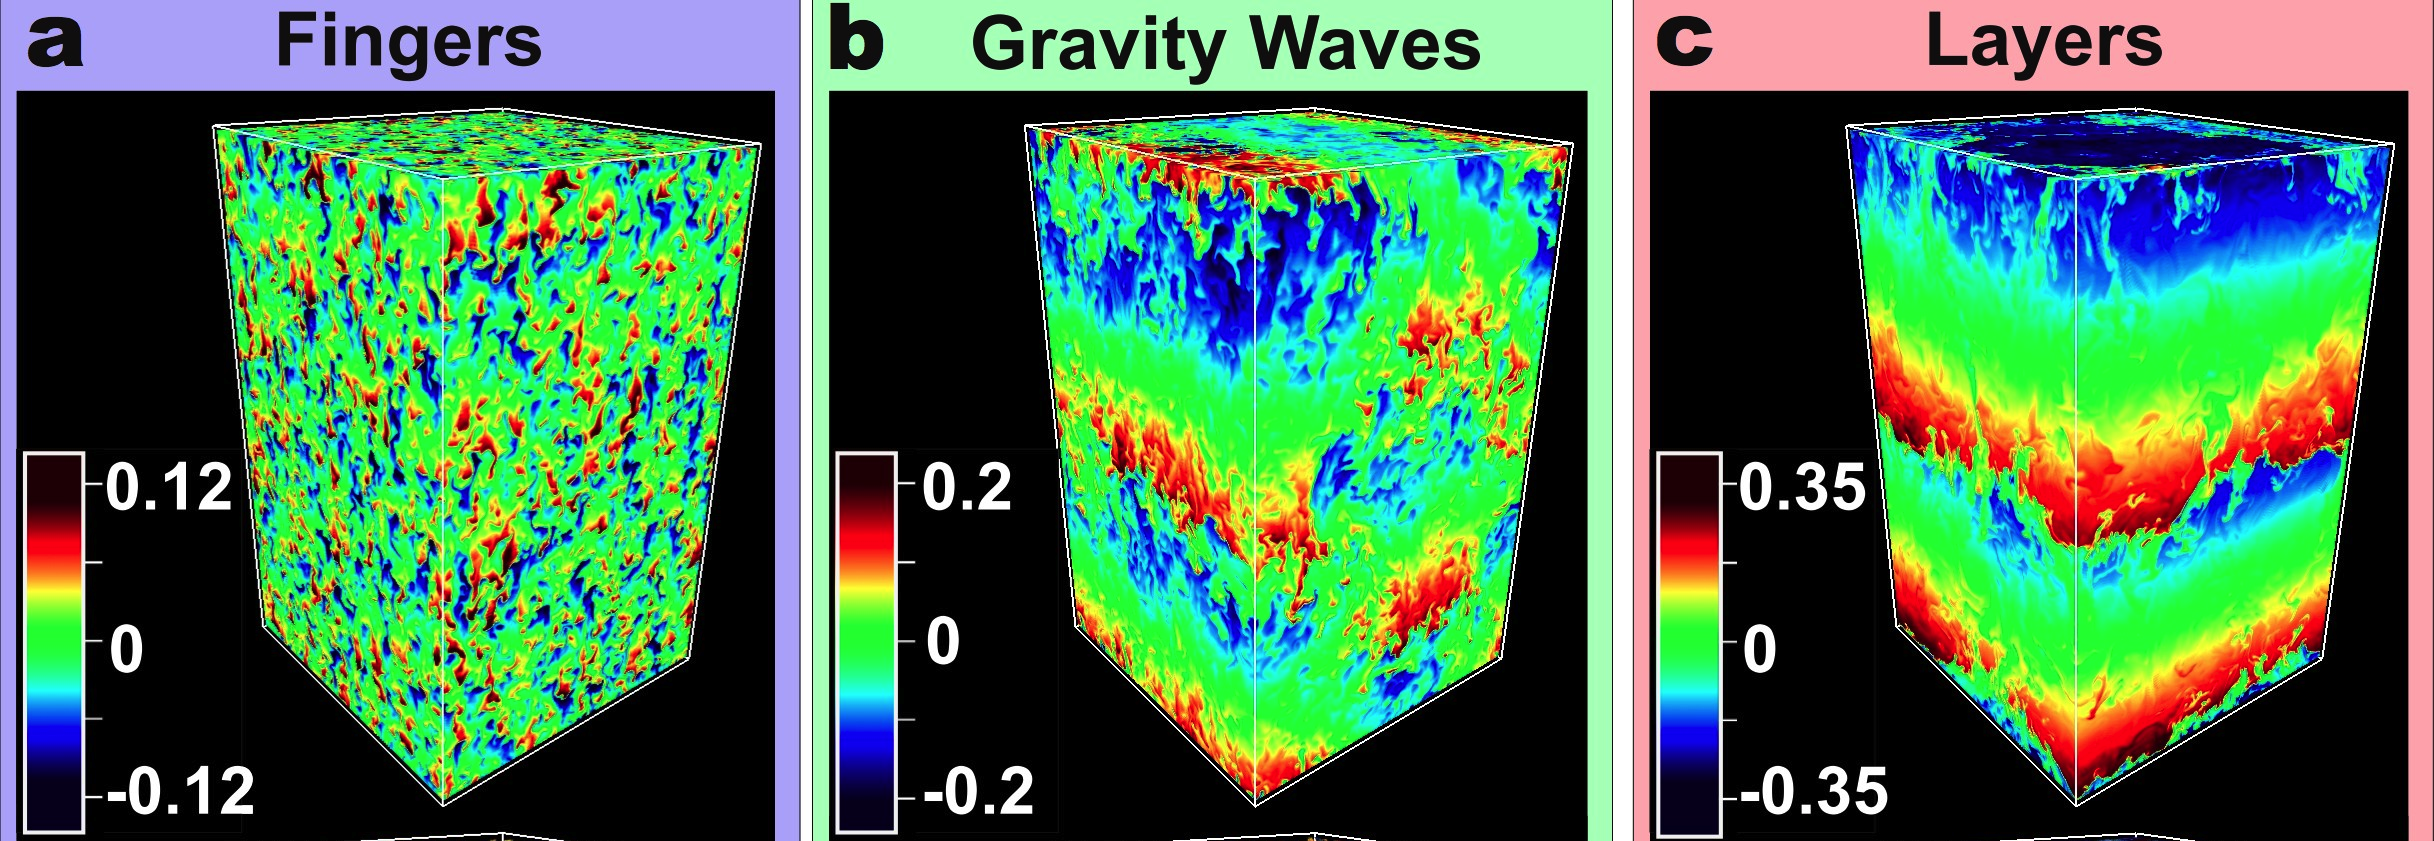
\includegraphics[width=\columnwidth]{layers.png}~\footnote{$\tilde{\mu}$ from \citep{Stellmach2011}}
% \end{figure}
% }

% \frame{\frametitle{We used an argument of shearing stress causing saturation to explain the fluxes.}
% \begin{figure}
% \subfloat[Fingers]{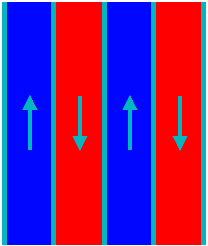
\includegraphics[height=75pt]{pngs/elevator_diagram.png}}
% \subfloat[Shearing]{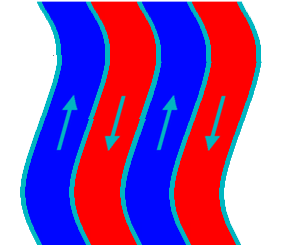
\includegraphics[height=75pt]{pngs/shear_diagram.png}}
% \end{figure}
% }

% \frame{\frametitle{We were able to use this to construct a semi-analytic model that accurately fit our results.}
% \begin{figure}[h]
% 	\includegraphics[height=.9\textwidth,angle=270]{figs/fgm_mu_talk.eps}
% \end{figure}
% }

\frame{\frametitle{Depending on the strength of the gradients, double- diffusive convection can take the form of  convective layers.}
	\begin{figure}[h]
		\centering
		\includegraphics[width=1\textwidth]{../figs/layer-merge.png}\footnote{\citep{Wood2013}}
	\end{figure}
}

\frame{\frametitle{In Boussinesq simulations, these layers merge until they fill the domain, but in reality, they reach an equilibrium.}
\begin{figure}[h]
	\centering
	\includegraphics[width=1\textwidth]{../figs/layer-merge.png}\footnote{\citep{Wood2013}}
\end{figure}
}

% \frame{\frametitle{To determine which regime is relevant to stars, we look at the condition for layer formation from \citet{Mirouh2012}.}
% 	\begin{figure}[h]
% 		\centering
% 			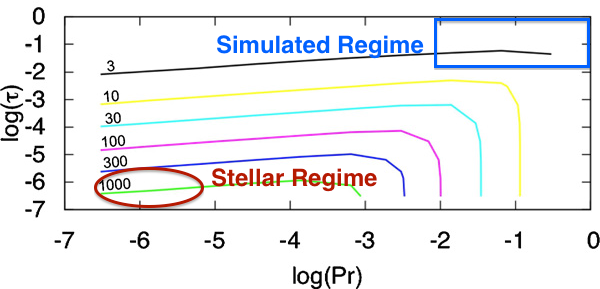
\includegraphics[width=0.9\textwidth]{../pngs/layer_condition.png}\footnote{\citep{Mirouh2012}}
% 			\caption{$R_{L}^{-1}$, the maximum $R_{0}^{-1}$ for which layers exist}
% 		\label{fig:pngs_layer_condition}
% 	\end{figure}
% }

% \frame{\frametitle{We find in KEPLER simulations that semi-convection regions exist preferentially in the layer-forming regime.}
% \begin{figure}[h]
% 	\centering
% 		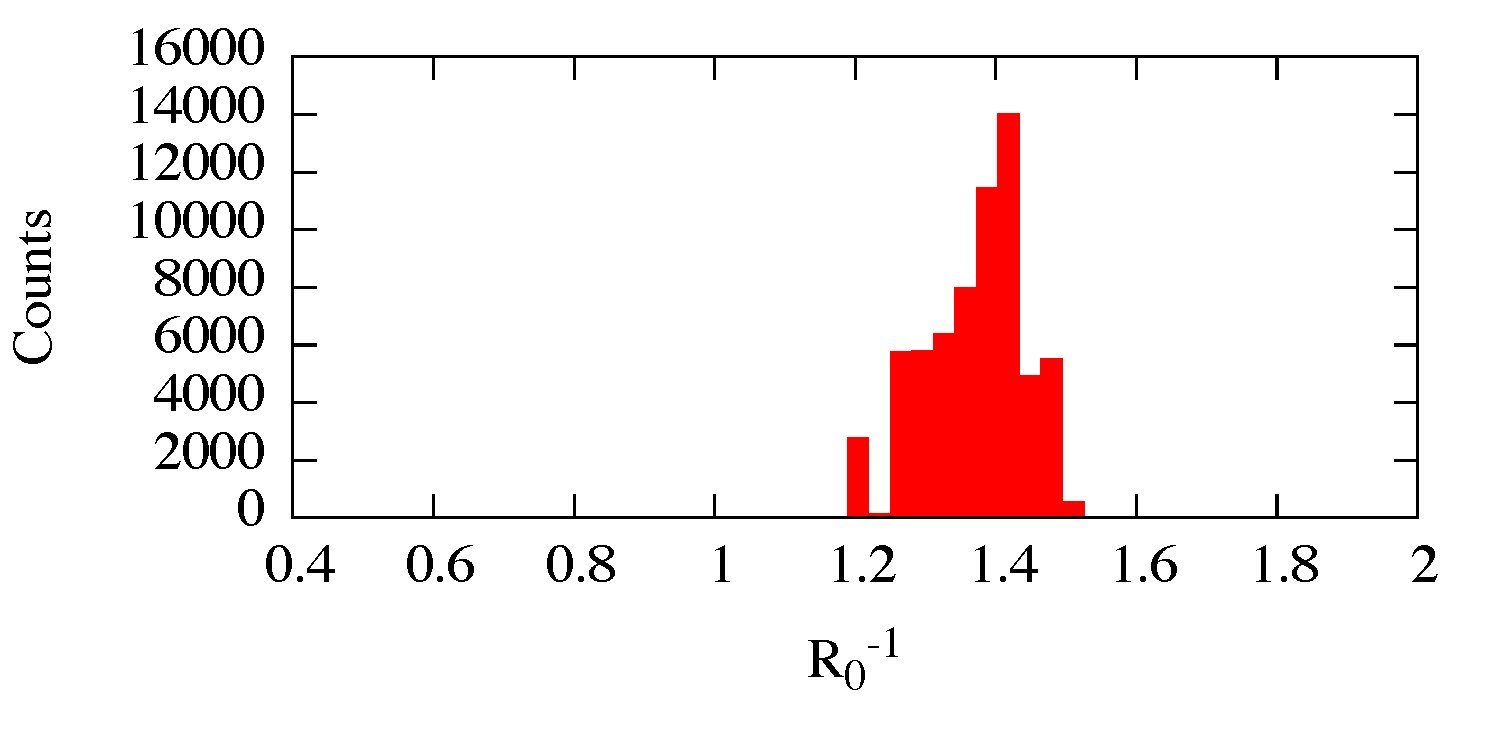
\includegraphics[width=.9\textwidth]{figs/r0hist.pdf}
% 	\caption{For semi-convection to be in the layered regime, $1<R_{0}^{-1}<R_{L}^{-1}\sim1000$} 
% 	\label{fig:figs_r0hist}
% \end{figure}
% }

% \subsection{Model}

% \frame{\frametitle{\citet{Wood2013} determined an empirical model for the fluxes in layers with one free parameter, $l_{\rm{semi}}$.}
% 	\begin{figure}[h]
% 		\centering
% 			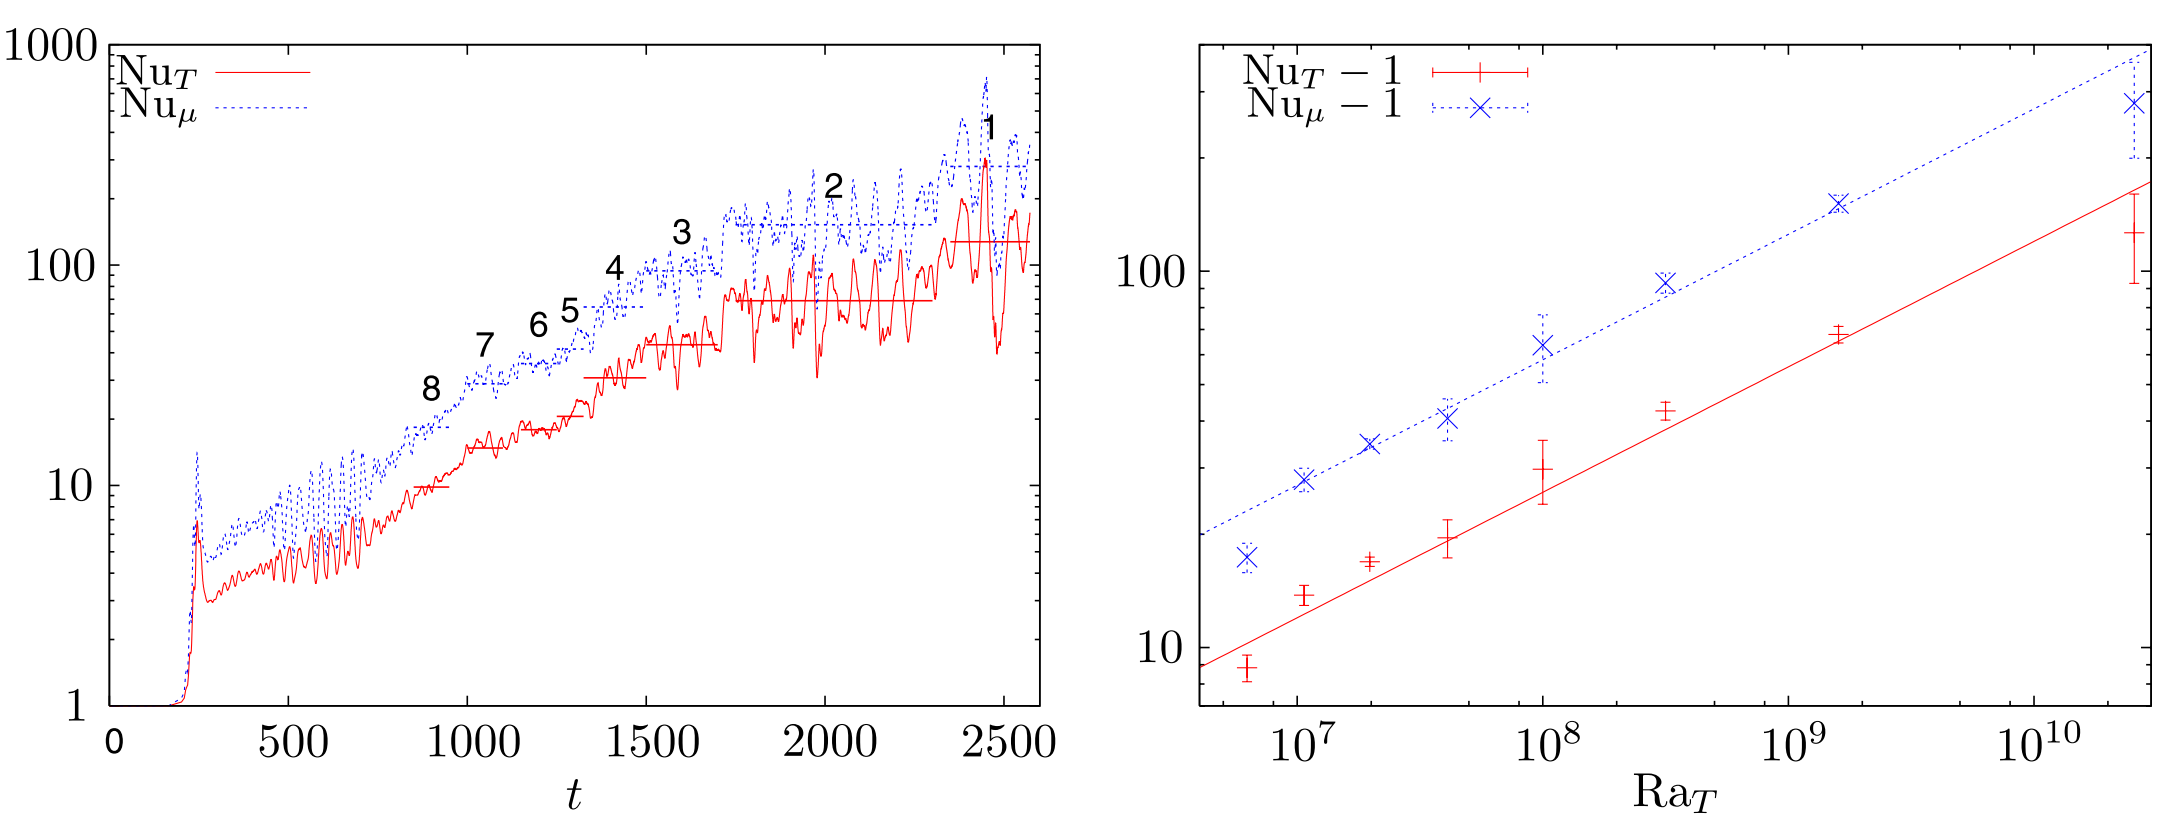
\includegraphics[width=.9\textwidth]{figs/wood-layers.png}\footnote{\citep{Wood2013}}
% 		\label{fig:figs_wood-layers}
% 	\end{figure}
% \begin{overprint}
% 	\only<1>{\begin{equation}
% Q_{\rm{semi}}=-0.1\left(\frac{g\delta|\frac{dT}{dr}-\left.\frac{dT}{dr}\right|_{\rm ad}|(l_{\rm semi})^{4}}{T\kappa_{T}^{2}}\right)^{1/3}\rho{c_{p}}\kappa_{T}\left(\frac{dT}{dr}-\left.\frac{dT}{dr}\right|_{\rm ad}\right)
% \end{equation}}
% \only<2>{\begin{equation}
% 		\kappa_{\mu, {\rm semi}}=0.03\left(\nu\kappa_{T}^{3}\right)^{1/4}\left(\frac{g\delta|\frac{dT}{dz}-\left.\frac{dT}{dz}\right|_{\rm ad}|(l_{\rm semi})^{4}}{\nu T\kappa_{T}}\right)^{0.37}
% 	\end{equation}}
% \end{overprint}
% }

% \frame{\frametitle{The Boussinesq approximation does not constrain the layer height; layers merge until they fill the domain.}
% \begin{figure}[h]
% 	\centering
% 		\includegraphics[width=.9\textwidth]{figs/layer-merge.png}\footnote{\citep{Wood2013}}
% 	\label{fig:figs_layer-merge}
% \end{figure}
% }

% \frame{\frametitle{We'd like to perform a new series of simulations to determine the maximum height of these layers.}
% \begin{itemize}
% 	\item Cover new physics not present in PADDI
% 	\begin{itemize}
% 		\item Non-linear diffusion
% 		\item Pseudo-incompressibility 
% 	\end{itemize}
% 	\item Attempt larger domains
% 	\begin{itemize}
% 		\item Move to 2D for this to be feasible
% 	\end{itemize}
% 	\item Finely resolve only layer interfaces
% 	\begin{itemize}
% 		\item Not possible in a traditional spectral code!
% 	\end{itemize}
% \end{itemize}
% }